% Talk for the ACL2 Workshop 2026, 25 minutes.
%
% Build the slides:          latexmk -pdf slides.tex
% Build the speaker notes:   latexmk -pdf slides-notes.tex
%   (one page per slide: a thumbnail of the slide and its notes)
%
% Speaker notes are the \note{...} blocks at the end of each frame.
\documentclass[aspectratio=169,10pt]{beamer}

\usepackage[T1]{fontenc}
\usepackage[utf8]{inputenc}
\usepackage{lmodern}
\usepackage{amsmath,amssymb}
\usepackage{booktabs}
\usepackage{listings}
\usepackage{tikz}
\usetikzlibrary{arrows.meta,positioning,shapes.geometric,calc}

\setbeamertemplate{navigation symbols}{}
\setbeamertemplate{footline}[frame number]
\ifdefined\withnotes
  \setbeameroption{show only notes}
  \setbeamertemplate{note page}[plain]
  \setbeamerfont{note page}{size=\small}
  % Notes pages: slide thumbnail on top, then the notes.
  \setbeamertemplate{note page}{%
    \vspace{0.5ex}%
    \begin{center}\insertslideintonotes{0.38}\end{center}%
    \vspace{0.5ex}%
    {\usebeamerfont{note page}\insertnote\par}}
\fi

% ---------------------------------------------------------------- listings
\lstdefinelanguage{acl2}{
  morekeywords={define,defrule,defruled,defun-sk,defequiv,defcong,defconst,
    forall,implies,and,or,not,iff,
    if,let,let*,b*,cond,equal,list,cons,car,cdr,cadr,caddr,append,atom,
    unless,natp,zp,null,consp,t,nil,assert-event},
  sensitive=false,
  morecomment=[l]{;},
  morestring=[b]",
  alsoletter={-*?<>=:},
}
\lstset{
  language=acl2,
  basicstyle=\ttfamily\footnotesize,
  keywordstyle=\color{blue!60!black}\bfseries,
  commentstyle=\color{gray}\itshape,
  columns=fullflexible,
  keepspaces=true,
  showstringspaces=false,
  escapeinside={(*@}{@*)},
}
\newcommand{\code}[1]{\texttt{#1}}
\newcommand{\F}{\mathbb{F}_2}
\newcommand{\M}{\mathcal{M}^{(n)}}

% ---------------------------------------------------------------- title
\title[Flip Graph Connectivity in ACL2]{Formalizing the Connectivity Theorem for the\\
  Matrix Multiplication Flip Graph in ACL2}
\author{Quan Luu \and Zeke Medley \and Panagiotis Manolios}
\institute{Northeastern University}
\date{ACL2 Workshop 2026}

\begin{document}

\begin{frame}
  \titlepage
  \note{
    \textbf{[0:00]} Hi, I'm Quan. This is joint work with Zeke Medley and
    Pete Manolios at Northeastern.

    The theorem is that the matrix multiplication flip graph over $\F$ is
    strongly connected. But this talk is not a tour of the proof. The proof
    comes from our companion ALENEX paper, and turning it into ACL2 was
    mostly translation. What I want to talk about are the
    decisions we made along the way, the places where the paper proof did
    not translate directly, and a few things we added that the paper did not
    ask for. At the end, some lessons from doing this with an LLM.
  }
\end{frame}

% ================================================================ Motivation
\section{Motivation}

\begin{frame}{Fast matrix multiplication and the flip graph}
  \begin{itemize}
    \item A \alert{scheme} computes the product of two $n\times n$ matrices;
      its \alert{rank} is the number of scalar multiplications.
    \item Recent records over $\F$, mostly found by \alert{searching the
      flip graph} (Kauers \& Moosbauer, 2023):
      \begin{center}
        \begin{tabular}{lcccc}
          \toprule
          format & $4\times4$ & $5\times5$ & $6\times6$ & $7\times7$ \\
          \midrule
          best rank & 47 & 93 & 153 & 245 \\
          naive     & 64 & 125 & 216 & 343 \\
          \bottomrule
        \end{tabular}
      \end{center}
    \item Vertices: schemes. Edges: local rewrites that keep what the scheme
      computes. Search walks from a known scheme toward lower rank.
    \item \alert{Which schemes can a search reach?}
      \begin{itemize}
        \item Arai et al.\ (2024): strongly connected with flip, plus and
          reduction edges, but the proof has a gap.
        \item Medley et al.\ (ALENEX 2027): over $\F$, \alert{flip and plus
          alone} suffice.
      \end{itemize}
  \end{itemize}
  \note{
    \textbf{[0:45]} Quick motivation. A scheme is a way to multiply
    matrices, and its rank is how many scalar multiplications it uses.
    Over $\F$ there has been a run of new records in the last few years,
    like 47 for four by four and 245 for seven by seven, and most of them
    were found by searching the flip graph. Its vertices are schemes, and
    its edges rewrite a scheme without changing what it computes.

    So the natural question for search is which schemes you can reach.
    Arai et al.\ showed strong connectivity, but with expensive reduction
    edges that searches usually leave out, and their main procedure relies
    on an invariant that is never established. Our companion paper shows
    that over $\F$ flip and plus edges alone are enough. Given that history,
    a machine-checked proof seemed worth having.
  }
\end{frame}

\begin{frame}{Schemes, flips and pluses in one slide}
  \begin{itemize}
    \item A \alert{scheme}: a multiset of nonzero rank-one tensors
      $A\otimes B\otimes C$ ($A,B,C\in\F^{n\times n}$) whose sum is the
      matrix multiplication tensor $\M$.
    \item Summand $r$ = one multiplication:
      $m_r = (\sum A^{(r)}_{gh}D_{gh})(\sum B^{(r)}_{ij}F_{ij})$,
      added into the entries of $DF$ where $C^{(r)}$ is 1.
  \end{itemize}
  \vspace{1ex}
  Edges, at position $A$ (and likewise $B$, $C$), with zero summands deleted:
  \begin{align*}
    \textbf{flip:}\quad & A\otimes B\otimes C,\ A\otimes B'\otimes C'
      \;\to\; A\otimes B\otimes (C+C'),\ A\otimes (B'+B)\otimes C' \\
    \textbf{plus:}\quad & A\otimes B\otimes C,\ A'\otimes B'\otimes C'
      \;\to\; A\otimes B\otimes C,\ (A'+A)\otimes B'\otimes C',\ A\otimes B'\otimes C'
  \end{align*}
  \vfill
  Over $\F$: subtraction is addition, and $X + X = 0$.
  So \alert{two identical summands cancel}.
  \note{
    \textbf{[2:00]} The one slide of background. A scheme is a multiset
    of rank-one tensors $A \otimes B \otimes C$ summing to the matrix
    multiplication tensor. Each summand is one multiplication: a linear
    form in $D$ times a linear form in $F$, added into the output entries
    where $C$ has a 1.

    A flip takes two summands that agree in one position and moves
    material between the other two. A plus splits one summand using
    another. Both preserve the sum.

    The single fact about $\F$ that the whole proof runs on: $X + X = 0$.
    Two identical summands cancel, and a flip of a summand with itself
    deletes the pair.
  }
\end{frame}

\begin{frame}{The proof at a glance (not the subject of this talk)}
  \begin{center}
  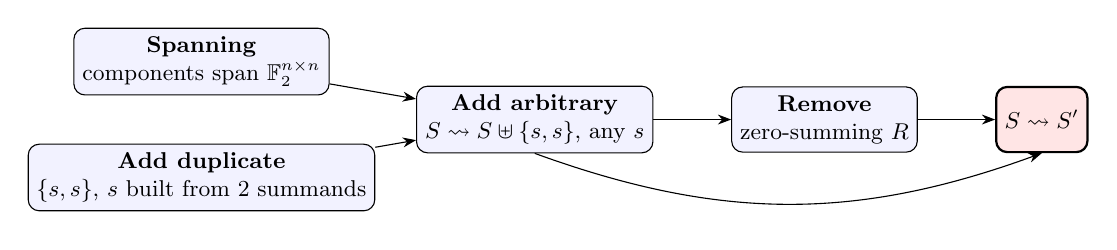
\begin{tikzpicture}[scale=0.92, transform shape,
      node distance=6mm and 9mm,
      box/.style={draw, rounded corners, align=center, font=\small,
                  minimum height=9mm, fill=blue!5},
      main/.style={box, fill=red!10, thick},
      >={Stealth}]
    \node[box] (span) at (0,0.8) {\textbf{Spanning}\\ components span $\F^{n\times n}$};
    \node[box] (dup) at (0,-0.8) {\textbf{Add duplicate}\\ $\{s,s\}$, $s$ built from 2 summands};
    \node[box] (arb) at (4.6,0) {\textbf{Add arbitrary}\\ $S \leadsto S\uplus\{s,s\}$, any $s$};
    \node[box] (zero) at (8.6,0) {\textbf{Remove}\\ zero-summing $R$};
    \node[main] (thm) at (11.6,0) {$S \leadsto S'$};
    \draw[->] (span) -- (arb);
    \draw[->] (dup) -- (arb);
    \draw[->] (arb) -- (zero);
    \draw[->] (zero) -- (thm);
    \draw[->] (arb.south) to[bend right=20] (thm.south);
  \end{tikzpicture}
  \end{center}
  \vspace{1ex}
  \[
    S \;\xrightarrow{\text{add each } s\in S' \text{ twice}}\;
      S \uplus S' \uplus S'
      \;\xrightarrow{\text{remove } S\uplus S'\text{, which sums to } \M+\M=0}\; S'
  \]
  \vfill
  \begin{block}{In ACL2}
    29 books, 215 definitions, 791 theorems; no trust tags,
    \code{skip-proofs} or \code{defaxiom}.
  \end{block}
  \note{
    \textbf{[3:00]} Here is the whole proof in one picture, so you know
    where things fit. You can add two copies of any summand you like: first
    from two existing summands, then, using spanning, anything at all. You
    can remove any submultiset that sums to zero. So from $S$, add two
    copies of everything in $S'$, then remove $S \uplus S'$, which sums to
    $\M + \M = 0$, and $S'$ is left.

    In ACL2 this is 29 books, 215 definitions and 791 theorems, with no
    trust tags or skip-proofs. I won't walk through it lemma by lemma.
    Instead, four things: how we set up types, how every lemma is stated,
    the spanning lemma, which didn't translate, and schemes versus
    algorithms.
  }
\end{frame}

% ================================================================ Decisions
\section{Design decisions}

\begin{frame}[fragile]{Decision 1: two recognizers for every type}
  \begin{columns}[T]
    \begin{column}{0.45\textwidth}
      \alert{Structural}: no size. Used in guards and \code{:returns}.
\begin{lstlisting}
(define bit-list-p (x)
  (if (atom x)
      (null x)
    (and (bitp (car x))
         (bit-list-p (cdr x)))))
\end{lstlisting}
    \end{column}
    \begin{column}{0.5\textwidth}
      \alert{Dimensioned}: fixes the size. Used in theorems.
\begin{lstlisting}
(define bit-listnp (x (n natp))
  (if (zp n)
      (null x)
    (and (consp x)
         (bitp (car x))
         (bit-listnp (cdr x) (1- n)))))
\end{lstlisting}
    \end{column}
  \end{columns}
  \vspace{1ex}
  Every operation has the same shape:
\begin{lstlisting}
(define bit-list-add ((x bit-list-p) (y bit-list-p))   ; structural guard
  :returns (z bit-list-p)                              ; structural :returns
  ...)
(defrule bit-listnp-of-bit-list-add                    ; separate size theorem
  (implies (and (bit-listnp x n) (bit-listnp y n))
           (bit-listnp (bit-list-add x y) n)))
\end{lstlisting}
  \note{
    \textbf{[4:00]} The first decision is about types. Every type has two
    recognizers. \code{bit-list-p} is structural: a true list of bits, any
    length. \code{bit-listnp} fixes the length to $n$. Matrices,
    summands and lists of matrices get the same two tiers.

    Why both? Most operations, like \code{bit-list-add}, take no dimension
    argument, so their guards and \code{:returns} \emph{can't} mention
    $n$; the structural recognizer is all that fits there, and it's exactly
    what guard verification needs, since \code{bitxor} wants integers. But
    ``the result is a bit list'' is too weak for any real proof. The proofs
    are about objects of the same size: two $n$-vectors, three $n \times n$
    factors, a tensor of $n^6$ bits. So every operation comes with a
    separate size theorem stated with the dimensioned recognizer.
  }
\end{frame}

\begin{frame}[fragile]{Decision 1, continued: what the two tiers buy}
  \begin{itemize}
    \item Guards stay cheap and dimension-free; theorems say what proofs need.
    \item The tiers are tied together:
      \code{(bit-listnp x (len x))} $\iff$ \code{(bit-list-p x)}.
    \item Nonzero-ness is a third layer, used only where it matters:
\begin{lstlisting}
(define summandp (s (n natp))
  (and (mat-triplep s)                       ; structural
       (bit-matp (car s) n n)                ; dimensioned
       (bit-matp (cadr s) n n)
       (bit-matp (caddr s) n n)
       (not (summand0p s n))))               ; nonzero
\end{lstlisting}
      \code{summand-dimp} is \code{summandp} without the last line: the
      spanning layer handles lists whose factors may be zero.
    \item Truncating operations: \code{bit-list-add} stops at the shorter
      list, so commutativity and associativity need \alert{no hypotheses}.
  \end{itemize}
  \note{
    \textbf{[5:15]} A few consequences. Guards stay simple and
    dimension-free, and the theorems carry the information the proofs
    actually use. The two tiers are tied together by one theorem: a list
    has dimension its own length exactly when it is structurally a bit
    list.

    Being nonzero is a third layer on top. \code{summandp} is structural,
    plus dimensioned, plus no zero factor. The spanning part of the proof
    works with lists of summands that may contain zero factors, so it uses
    \code{summand-dimp}, which is the same thing without the nonzero line.

    And a small trick: \code{bit-list-add} truncates to the shorter
    argument, so its algebra holds with no hypotheses at all. That keeps
    a lot of rewriting free.
  }
\end{frame}

\begin{frame}[fragile]{Decision 2: let the representation absorb the side conditions}
  \begin{itemize}
    \item A scheme is an \alert{ordered bag} (\code{std/obags}): sorted by
      \code{<<}, repeats allowed.
      \begin{itemize}
        \item Equal multisets are \code{equal}: no permutation reasoning.
        \item A move on two copies of the same summand needs multiplicity 2,
          not just membership.
      \end{itemize}
    \item ``With any zero summands deleted'' is built into insertion:
\begin{lstlisting}
(define insert-all-nonzero ((l mat-triple-listp) (s obag::bagp) (n natp))
  (if (atom l)
      s
    (if (summand0p (car l) n)
        (insert-all-nonzero (cdr l) s n)
      (obag::insert (car l) (insert-all-nonzero (cdr l) s n)))))
\end{lstlisting}
    \item Zero summands are excluded twice: \code{summandp} rejects them,
      insertion drops them. So the lemmas need \alert{no hypotheses ruling
      out degenerate cases}.
      \begin{itemize}
        \item e.g.\ adding a duplicate sum $X = A_1 + A_2$ needs no
          $X \neq 0$: if $X = 0$ the path is empty and both sides are $S$.
      \end{itemize}
  \end{itemize}
  \note{
    \textbf{[6:15]} Second decision: wherever possible, push side
    conditions into the representation instead of the theorems.

    Schemes are ordered bags from \code{std/obags}. Two schemes are equal
    as multisets exactly when they are \code{equal}, so we never reason
    about permutations or occurrence counts in statements. One subtlety:
    a bag doesn't distinguish occurrences, so when a move uses the same
    summand twice, validity asks for multiplicity two, not membership.

    The paper's definition of the moves ends with ``any zero summands
    deleted''. We make that the only way to insert. The payoff is that
    degenerate cases disappear from the lemmas. For example, adding a
    duplicate sum $X = A_1 + A_2$: if $X$ is zero, the path is empty, and
    the two zero summands we claim to add are dropped, so both sides are
    the original scheme. The theorem has no $X \neq 0$ hypothesis.
  }
\end{frame}

\begin{frame}[fragile]{Decision 3: paths are computed, never claimed}
\begin{lstlisting}[basicstyle=\ttfamily\small]
(defrule flip-plus-connectivity
  (implies (and (correct-schemep sch n)
                (correct-schemep sch2 n)
                (natp n) (<= 2 n))
           (b* ((path (main-path sch sch2 n))
                (res  (apply-moves path sch n)))
             (and (path-validp path sch n)
                  (equal res sch2)))))
\end{lstlisting}
  \vfill
  \begin{itemize}
    \item ``There is a path'' $\to$ a function \code{main-path} that
      \alert{returns} one. No \code{defun-sk}, no existential.
    \item \code{correct-schemep}: a bag of \code{summandp}s whose
      \code{scheme-sum} is \code{(mm-tensor n)}.
    \item \code{correct-schemep-of-apply-moves}: any valid path preserves
      correctness (over $\F$, deleting a summand changes the sum the way
      inserting it does).
  \end{itemize}
  \note{
    \textbf{[7:30]} Third decision, and the one that shaped everything
    else. The theorem says ``there is a path''. We never state that. We
    define a function, \code{main-path}, that computes the path from the
    two schemes, and the theorem says the path is valid and applying it
    gives you the second scheme. No \code{defun-sk}, no existential
    quantifier anywhere in the statement.

    Validity of a path is just the moves being legal one after another.
    And there's one basic invariant: a valid path preserves correctness.
    The proof is nice over $\F$: deleting a summand changes the sum
    exactly as inserting it would, so each move is handled by linearity.
  }
\end{frame}

\begin{frame}[fragile]{Decision 3, continued: an invariant theorem at every step}
  Every lemma: a \alert{path function}, and a theorem saying the path is
  valid and \alert{naming the scheme it lands on}.
\begin{lstlisting}
(defrule graft-invariant
  (implies (and (correct-schemep sch n) (natp n) (<= 2 n)
                (summand-listp l n))
           (b* ((path (graft-path sch l n))
                (res  (apply-moves path sch n)))
             (and (path-validp path sch n)
                  (equal res (insert-list l (insert-list l sch)))   ; S + l + l
                  (correct-schemep res n)))))
\end{lstlisting}
  \begin{itemize}
    \item Same shape for \code{add-duplicate}, \code{grow-chain-invariant},
      \code{add-arbitrary}, \code{decompose-pos-invariant},
      \code{zero-subset}, \dots
    \item Naming the destination is what lets one lemma
      \alert{hand its result to the next}.
    \item The main theorem: instantiate \code{graft-invariant}, then
      \code{zero-subset}. \alert{No induction.}
  \end{itemize}
  \note{
    \textbf{[8:30]} Every lemma follows that pattern. Here's
    \code{graft-invariant}, the first half of the main path: add two copies
    of each summand of a list. The conclusion has three parts: the path is
    valid, the result is \emph{equal} to an explicitly named scheme, here
    $S$ plus two copies of $l$, and that scheme is correct.

    The middle part is the key. Because each theorem names exactly where
    you end up, the next lemma's hypotheses are about a known term, and
    the lemmas just compose. The main theorem is two instantiations: graft,
    then remove the zero-summing part. No induction at the top level.
    Induction only happens inside lemmas, on the thing they iterate over,
    like the chain or the list of summands.
  }
\end{frame}

\begin{frame}[fragile]{Decision 3, consequence: compute the destination before the route}
  Paths are built \alert{before} any move is applied, so a later stage
  cannot observe the scheme an earlier stage produced. It must
  \alert{compute} it.
\begin{lstlisting}
(define zero-subset-path ((sch obag::bagp) (r mat-triple-listp) (n natp))
  (b* ((base (delete-list r sch))
       (l1 (expand-pos-list r 0 n))   (sch1 (insert-list l1 base))
       (l2 (expand-pos-list l1 1 n))  (sch2 (insert-list l2 base))
       (l3 (expand-pos-list l2 2 n))  (sch3 (insert-list l3 base)))
    (append (decompose-list-pos-path sch  r  0 n)
            (append (decompose-list-pos-path sch1 l1 1 n)
                    (append (decompose-list-pos-path sch2 l2 2 n)
                            (delete-pairs-path sch3 l3 n))))))
\end{lstlisting}
  \begin{itemize}
    \item \code{expand-pos-list} is the \alert{destination}, the path is the
      \alert{route}, and the invariant theorem says the route arrives.
  \end{itemize}
  \note{
    \textbf{[9:30]} One consequence I didn't expect. Because a path is a
    value computed up front, a later stage can't look at the scheme an
    earlier stage produced; it has to compute it.

    Removing a zero-summing set works in four stages: break every summand
    into unit matrices in position A, then B, then C, then delete the
    resulting identical pairs. The B sweep needs to know what the list
    looks like after the A sweep. So there are two functions per stage:
    \code{expand-pos-list} computes the destination as a list of
    summands, with no moves involved, and \code{decompose-list-pos-path}
    computes the route. The invariant theorem is what connects them. This
    split, destination versus route, shows up all over the development.
  }
\end{frame}

\begin{frame}[fragile]{Decision 3, consequence: everything runs}
  Every construction is executable, so every one was \alert{run at $n=2$
  before it was proved}. From \code{overview-proof.lisp}:
\begin{lstlisting}
(assert-event
 (let* ((x '((1 1) (0 1))) (y '((0 1) (1 1))) (z '((1 0) (1 1)))
        (path0 (add-arbitrary-path *arb-std2* x y z 2))
        (schb  (apply-moves path0 *arb-std2* 2))
        (path  (main-path schb *arb-std2* 2)))
   (and (correct-schemep *arb-std2* 2)
        (equal (scheme-rank *arb-std2*) 8)       ; standard scheme
        (correct-schemep schb 2)
        (equal (scheme-rank schb) 10)            ; after adding a summand twice
        (path-validp path schb 2)
        (equal (apply-moves path schb 2) *arb-std2*))))   ; and back
\end{lstlisting}
  \begin{itemize}
    \item The \alert{statement} of the main theorem can be evaluated on
      concrete schemes before any proof exists.
    \item A wrong construction and a hard proof look different.
  \end{itemize}
  \note{
    \textbf{[10:30]} The other consequence is that everything runs. Paths
    are data, so every construction was run at $n = 2$ before we tried to
    prove anything about it. This is from the overview book: start from
    the standard rank-8 scheme, add some summand twice to get a correct
    rank-10 scheme, then run \code{main-path} back, and check that it's
    valid and lands exactly on the standard scheme.

    More than that, the conclusion of the main theorem is itself an
    executable term, so you can evaluate the theorem on concrete inputs
    before proving it. If it evaluates to false, the construction is
    wrong. If it's true and the proof is still failing, the proof is just
    hard. That distinction turned out to matter a lot, and I'll come back
    to it in the LLM part.
  }
\end{frame}

% ================================================================ Span
\section{The spanning lemma}

\begin{frame}{The spanning lemma does not translate directly}
  \begin{block}{Lemma (Spanning)}
    Let $S$ be a scheme for $\M$. Then the $A$-components of the summands
    of $S$ span the full space of $n\times n$ matrices.
  \end{block}
  \vspace{1ex}
  Three problems:
  \begin{enumerate}
    \item ``Span'' is an \alert{existential}: some linear combination
      exists. A path cannot be built from an existence statement.
    \item The proof needs \alert{more} than spanning. To add
      $X\otimes\cdot\otimes\cdot$, it walks a chain
      \[
        A_0 \to A_0 + A(u_1) \to \dots \to X
      \]
      and \alert{every partial sum must be nonzero}, or the carried summand
      vanishes.
    \item The paper splits into \alert{two cases} on whether $A_0$ appears
      in the expansion of $X$.
  \end{enumerate}
  \note{
    \textbf{[11:30]} Now the part of the proof that didn't translate. The
    spanning lemma says the A-components of a correct scheme span the
    whole matrix space. On paper that's one line, but there are three
    problems.

    First, ``span'' means ``there exists a linear combination''. We just
    decided that paths are computed, and you can't compute a path from an
    existence statement.

    Second, the proof needs more than spanning. To get a summand with
    A-component $X$, it walks from some existing $A_0$ toward $X$, adding
    one A-component at a time, and every intermediate sum has to be
    nonzero. Otherwise the summand being carried has a zero factor and
    disappears.

    Third, the informal proof splits into two cases depending on whether
    $A_0$ itself is needed in the expansion of $X$.
  }
\end{frame}

\begin{frame}[fragile]{Step 1: state the lemma with the witness}
  Don't prove a combination exists; \alert{compute} it and prove what it
  computes.
\begin{lstlisting}
(defrule span-lemma
  (implies (and (correct-schemep sch n) (natp n) (< 0 n)
                (natp i) (natp j) (natp k) (< i n) (< j n) (< k n))
           (equal (a-witness-sum sch i j k n)
                  (bit-mat-unit i j n n))))
\end{lstlisting}
  \begin{itemize}
    \item \code{a-witness-sum}: add the $A$-factors of the summands with
      $B[j,k]\cdot C[i,k] = 1$. The result is the unit matrix $E_{ij}$.
    \item Proof by entries, against the entry law of \code{mm-tensor}
      (every fact about matrix multiplication comes from that one theorem).
    \item Matrix equality from entry equality, \alert{without quantifiers}:
      \code{mat-diff-pos} computes the first position where two matrices
      differ, and \code{mat-diff-pos-correct} says unequal matrices differ
      there.
  \end{itemize}
  \note{
    \textbf{[12:45]} Step one: state the lemma with the witness. For each
    unit matrix $E_{ij}$ and any $k$, \code{a-witness-sum} picks out the
    summands whose $B[j,k]$ times $C[i,k]$ is 1 and adds their A-factors.
    On a correct scheme, that sum is exactly $E_{ij}$. Since unit matrices
    span everything, that's spanning, but with the combination written
    down.

    The proof reads entries off the tensor using a single entry law for
    \code{mm-tensor}; every fact about matrix multiplication in the
    development comes from that one theorem.

    One small thing I like: to go from ``equal at every entry'' to
    ``equal matrices'' we didn't want a quantified extensionality
    principle either. \code{mat-diff-pos} computes the first position
    where two matrices differ, and the theorem says that if they're
    unequal, they really differ there. Then you argue by contraposition.
  }
\end{frame}

\begin{frame}[fragile]{Step 2: span membership as a recursive, executable predicate}
  Over $\F$ the only coefficients are 0 and 1, so the span is the set of
  \alert{subset sums}:
\begin{lstlisting}
(define in-spanp ((x bit-list-listp) (mats bit-mat-list-p) (m natp) (n natp))
  (if (atom mats)
      (equal x (bit-mat0 m n))
    (or (in-spanp x (cdr mats) m n)                         ; skip it
        (in-spanp (bit-mat-add x (car mats)) (cdr mats) m n))))  ; use it

(define span-witness (x mats m n)        ; same recursion, records the choice
  (if (atom mats) nil
    (if (in-spanp x (cdr mats) m n)
        (cons 0 (span-witness x (cdr mats) m n))
      (cons 1 (span-witness (bit-mat-add x (car mats)) (cdr mats) m n)))))
\end{lstlisting}
  \begin{itemize}
    \item \code{lincomb-of-span-witness}: if \code{x} is in the span, the
      bits reproduce \code{x}. Same recursion, so same induction.
    \item Exponential, and we don't care: we prove the construction, we
      don't run it at scale.
    \item Rejected: \code{defun-sk} (not executable, awkward to rewrite
      with); Gaussian elimination (more definitions and proof, for
      efficiency we don't need).
  \end{itemize}
  \note{
    \textbf{[14:00]} Step two: we needed span membership as something we
    could compute with. Over $\F$ coefficients are just 0 or 1, so being in
    the span means being a subset sum. \code{in-spanp} decides that
    recursively: for each matrix, either skip it, or use it and subtract it
    from the target.

    \code{span-witness} has the same recursion and records which branch
    was taken as a bit. Because the two functions recurse the same way,
    the correctness proof, that the bits add back up to $x$, is one
    induction.

    It's exponential. We were fine with that: we prove things about the
    construction, we don't run it on seven by seven. We did consider the
    alternatives. A \code{defun-sk} isn't executable and is awkward to
    rewrite with, and Gaussian elimination would be much more machinery
    for an efficiency we don't need.
  }
\end{frame}

\begin{frame}[fragile]{Step 3: from a span to a chain with nonzero partial sums}
  \begin{center}
  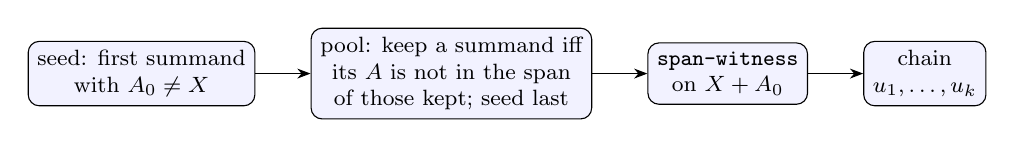
\begin{tikzpicture}[node distance=4mm and 7mm,
      box/.style={draw, rounded corners, align=center, font=\footnotesize, fill=blue!5},
      >={Stealth}]
    \node[box] (seed) {seed: first summand\\ with $A_0 \neq X$};
    \node[box, right=of seed] (pool) {pool: keep a summand iff\\ its $A$ is \alert{not in the span}\\ of those kept; \alert{seed last}};
    \node[box, right=of pool] (bits) {\code{span-witness}\\ on $X + A_0$};
    \node[box, right=of bits] (chain) {chain\\ $u_1,\dots,u_k$};
    \draw[->] (seed) -- (pool);
    \draw[->] (pool) -- (bits);
    \draw[->] (bits) -- (chain);
  \end{tikzpicture}
  \end{center}
  \begin{itemize}
    \item The pool is \alert{independent}: no element is in the span of
      the elements after it. So every partial sum is a nontrivial
      combination of independent matrices: \alert{nonzero}.
    \item The seed is \alert{last}: if the combination uses $A_0$, it uses
      it at the final step, where the running total is $X \neq 0$.
    \item The paper's two cases \alert{disappear}: they are handled by
      the order of the list.
  \end{itemize}
\begin{lstlisting}[basicstyle=\ttfamily\scriptsize]
;; n = 2, pool A-components (E00 E01 E10 E11), seed E11 last
(equal (arb-coeffs *arb-std2* x1 2) '(1 1 0 0))   ; X = E00+E01+E11: seed unused
(equal (arb-coeffs *arb-std2* x2 2) '(1 0 0 1))   ; X = E00: seed used, last
\end{lstlisting}
  \note{
    \textbf{[15:15]} Step three is where it got interesting. We need a
    chain of summands from the seed $A_0$ to $X$ with every partial sum
    nonzero. The construction: pick as seed the first summand whose A is
    not $X$. Then build a pool by walking the scheme and keeping a summand
    only if its A-component is not already in the span of what we've kept.
    That makes the pool independent. Put the seed last. Then run
    \code{span-witness} for $X + A_0$ over the pool, and the 1-bits are
    the chain.

    Independence gives nonzero partial sums: each one is a nontrivial
    combination of independent matrices. The only worry is the seed
    itself, and because it's last, if it's used at all, it's used at the
    very last step, where the running total is $X$, nonzero by assumption.

    So the paper's case split on the seed's coefficient just goes away;
    the order of the list handles it. The two runs at the bottom are the
    two cases at $n = 2$: one where the seed isn't used, one where it's
    used as the last link.
  }
\end{frame}

% ================================================================ Algorithms
\section{Schemes are algorithms}

\begin{frame}[fragile]{Beyond the main proof: are vertices really algorithms?}
  The main theorem is about \alert{schemes}. The claim that they
  \alert{are} multiplication algorithms was informal. We made it formal.
  \vspace{1ex}

  A small language of \alert{bilinear algorithms} (\code{matmul-expr.lisp}):
  \begin{itemize}
    \item linear forms: \code{(:var i j)}, \code{(:add e1 e2)},
      \code{(:scale b e)}
    \item an algorithm: $R$ products \code{(:mul d-form f-form)}, and an
      $n\times n$ table listing which products are summed into each output entry
    \item only bilinear algorithms are expressible, so \alert{rank is the
      right measure}
  \end{itemize}
\begin{lstlisting}[basicstyle=\ttfamily\scriptsize]
(defconst *strassen2*
  (cons (list (list :mul '(:add (:var 0 0) (:var 1 1)) '(:add (:var 0 0) (:var 1 1)))
              (list :mul '(:add (:var 1 0) (:var 1 1)) '(:var 0 0))
              ...)                                        ; 7 products
        '(((0 3 4 6) (2 4))                               ; output table
          ((1 3) (0 1 2 5)))))
\end{lstlisting}
\begin{lstlisting}
(defun-sk algo-correctp (alg n)
  (forall (d f) (implies (and (bit-matp d n n) (bit-matp f n n))
                         (equal (eval-algo alg d f n) (bit-mat-mul d f n)))))
\end{lstlisting}
  \note{
    \textbf{[16:45]} The last technical part is something we added that the
    connectivity proof doesn't need. Everyone says the vertices of the flip
    graph are matrix multiplication algorithms, and the main theorem is
    only interesting because of that. But in our development it's a theorem
    about bags of matrix triples. So we made the connection formal.

    We wrote a small language for bilinear algorithms: linear forms in the
    entries of one matrix, products of a form in $D$ with a form in $F$, and
    an output table saying which products go into each entry. A product of
    two forms in the same matrix can't be written, so only bilinear
    algorithms are expressible, which is what makes the number of products
    the right measure. Here's Strassen written in it. And an algorithm is
    correct if it returns the product on all inputs. This is the one place
    we use a quantifier, because it is genuinely ``for all inputs''.
  }
\end{frame}

\begin{frame}{Translation and conversion}
  \begin{center}
  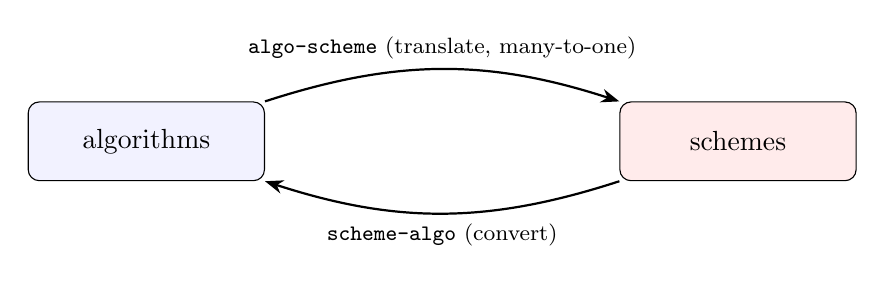
\begin{tikzpicture}[>={Stealth}, node distance=45mm]
    \node[draw, rounded corners, fill=blue!5, minimum width=30mm, minimum height=10mm] (A) {algorithms};
    \node[draw, rounded corners, fill=red!8, minimum width=30mm, minimum height=10mm, right=of A] (S) {schemes};
    \draw[->, thick] (A.north east) to[bend left=18] node[above, font=\footnotesize]{\code{algo-scheme} (translate, many-to-one)} (S.north west);
    \draw[->, thick] (S.south west) to[bend left=18] node[below, font=\footnotesize]{\code{scheme-algo} (convert)} (A.south east);
  \end{tikzpicture}
  \end{center}
  \begin{description}[Completeness]
    \item[Existence] the textbook algorithm translates to the standard scheme,
      correct for every $n$: \alert{the main theorem is not vacuous}
    \item[Soundness] correct scheme $\Rightarrow$ converted algorithm is correct
    \item[Completeness] correct algorithm $\Rightarrow$ correct scheme, of rank
      $\le$ the number of products
    \item[Round trip] \code{(algo-scheme (scheme-algo sch n) n)} $=$ \code{sch}
  \end{description}
  \vspace{1ex}
  \begin{itemize}
    \item Completeness needs only the $n^4$ pairs of \alert{unit inputs}:
      on $(E_{ab}, E_{cd})$ the output reads off one entry of the tensor
      (\code{agrees-on-unitsp}, executable).
    \item Soundness + completeness: our \code{mm-tensor}, defined as
      $\sum E_{ij}\otimes E_{jk}\otimes E_{ik}$, is the tensor defined by
      its action on $D$, $F$.
  \end{itemize}
  \note{
    \textbf{[18:00]} Two maps. Translation takes an algorithm to a scheme,
    one summand per product: the coefficient matrices of the two forms, and
    the output entries that product feeds. Conversion goes back.

    Four results. Existence: the textbook algorithm translates to the
    standard scheme, which is correct for every $n$, so the main theorem is
    never vacuously true. Soundness: a correct scheme converts to a correct
    algorithm. Completeness: a correct algorithm translates to a correct
    scheme, with rank at most its number of products. And the round trip:
    convert, then translate, and you get the same scheme back.

    The nice trick in completeness: you don't need all inputs. On a pair
    of unit matrices, the algorithm's output reads off exactly one entry of
    its tensor, so checking the $n^4$ unit pairs pins the tensor down.

    And a side benefit: we define \code{mm-tensor} as the explicit sum,
    not by its action on matrices. Soundness and completeness together say
    those two definitions agree.
  }
\end{frame}

\begin{frame}[fragile]{Schemes are equivalence classes of algorithms}
  Translation forgets the order of products, how a form is written,
  repeated indices (by parity), and zero products.
\begin{lstlisting}
(define scheme-equiv (a1 a2)
  (and (equal (algo-dim a1) (algo-dim a2))
       (equal (algo-scheme a1 (algo-dim a1))
              (algo-scheme a2 (algo-dim a2)))))
(defequiv scheme-equiv)
(defcong scheme-equiv equal (algo-canon alg) 1)   ; canonical representative

(assert-event (and (scheme-equiv *strassen2* *strassen2-rep*)   ; extra 2 2 cancels
                   (not (equal *strassen2* *strassen2-rep*))
                   (not (scheme-equiv *strassen2* *naive2*))))
\end{lstlisting}
  \begin{itemize}
    \item Classes are in \alert{bijection with schemes}; equivalent
      algorithms compute the same function.
    \item Finer than ``same function'': Strassen and the naive algorithm
      both multiply, but are not equivalent.
    \item So: \alert{any correct bilinear algorithm can be turned into any
      other by flips and pluses on its scheme.}
  \end{itemize}
  \note{
    \textbf{[19:15]} Translation is many-to-one. It forgets the order of
    the products, how each form is written, so $a + b$ and $b + a$ are the
    same, repeated indices in the output table by parity, and zero
    products. So two algorithms are equivalent if they translate to the
    same scheme. That's registered as a real ACL2 equivalence with
    \code{defequiv}, and the canonical representative, convert after
    translate, is a congruence.

    The example: Strassen, and Strassen with product 2 listed twice more
    in one output entry, which cancels. Different algorithms, same scheme.
    The naive algorithm is in a different class even though it computes
    the same function. So this is finer than extensional equality.

    The upshot: the vertices really are bilinear algorithms up to this
    equivalence, and the main theorem says you can get from any correct
    bilinear algorithm to any other with flips and pluses.
  }
\end{frame}

% ================================================================ LLM
\section{Working with a language model}

\begin{frame}{How the development was done}
  Claude, through Claude Code (mostly Fable 5; Opus 5 and Fable 5.1 for
  some sessions).
  \begin{enumerate}
    \item \alert{We} wrote the base: bit lists, bit matrices, their operations.
    \item The model proposed representations for summands, schemes, moves,
      paths. \alert{We} reviewed them and fixed the conventions: two-tier
      recognizers, \code{define} with \code{:returns}, \code{defrule}.
    \item The model formalized the rest: main theorem and all lemmas
      \alert{within two days}.
    \item \alert{We} asked it to explain what it built and why, and ordered
      changes (guard verification, restructuring books).
  \end{enumerate}
  \vfill
  \begin{block}{What it found most useful}
    ``In ACL2 everything runs. [\dots] In a prover where the statement
    cannot be run, I would have had no way to tell a wrong construction
    from a hard proof.''
  \end{block}
  \note{
    \textbf{[20:30]} Now, how this was actually built. We used Claude
    through Claude Code. We wrote the base library ourselves: bit lists,
    matrices, the operations. Then we gave the model the companion paper
    and asked it to propose representations. We reviewed those and fixed
    the conventions, including the two-tier recognizers from earlier.
    Then it formalized the rest, and within two days it had the main
    theorem and all the lemmas proved.

    After that, our job was mostly asking it to explain what it had built
    and why, and ordering changes when the explanation showed a problem:
    guard verification everywhere, dropping guards that weren't needed,
    restructuring the books.

    We asked it what helped most, and its answer was the point from
    earlier: everything runs. It found a wrong index convention in its
    first \code{mm-tensor} by running it at $n = 2$, in seconds instead
    of hours of failed proofs. Our takeaway: evaluate constructions and
    candidate theorem statements on small inputs before proving them.
  }
\end{frame}

\begin{frame}{The other direction: an unassisted run}
  A fresh session (Fable 5.1) got the companion paper \alert{and nothing
  else}: no conventions, no code, no feedback.
  \begin{itemize}
    \item 24 certified books covering the \alert{whole} paper.
    \item A \alert{simpler} chain: greedy, after cancelling duplicate pairs.
      No independent pool needed.
  \end{itemize}
  \begin{center}\small
    \begin{tabular}{lrrrrr}
      \toprule
      connectivity proof & books & lines & functions & theorems & cert.\ (serial) \\
      \midrule
      guided (this paper) & 19 & 6363 & 137 & 527 & 51\,s \\
      unassisted          &  9 & 3005 & 108 & 409 & 1240\,s \\
      \bottomrule
    \end{tabular}
  \end{center}
  \begin{itemize}
    \item The time gap: we \alert{disable definitions by default}; it did
      not. Six theorems and two termination proofs take 90\% of its time.
    \item \alert{Same theorem?} ACL2s random testing, $n = 2, 3$: each
      \code{main-path} works under the other's definitions. One convention
      difference found (flip at $B$, summands swapped).
  \end{itemize}
  \note{
    \textbf{[22:00]} We also ran it the other way: a fresh session with
    only the companion paper, and no code, conventions or feedback. It
    produced 24 certified books covering the whole paper, more than we
    formalized, including the rank-245 scheme.

    And it found a simpler chain construction than ours. Instead of the
    independent pool, it builds the chain greedily, always picking an
    element that differs from the running sum, after cancelling duplicate
    pairs. So all of step three that I just showed you has an easier
    alternative.

    Its connectivity proof is half the size of ours, but takes 24 times as
    long to certify. That's almost entirely because it leaves definitions
    enabled; six theorems and two termination proofs are 90 percent of
    the time.

    To check the two prove the same theorem, we used ACL2s random testing
    at $n = 2$ and 3. It found one real difference: the two encode the flip
    at position B with the summands swapped. Both are consistent with the
    definition. With the translation adjusted, everything agrees.
  }
\end{frame}

% ================================================================ Conclusion
\section{Conclusion}

\begin{frame}{Takeaways}
  \begin{itemize}
    \item \alert{Two recognizers per type}: structural for guards,
      dimensioned for theorems.
    \item \alert{Let the representation absorb side conditions}: obags,
      zero summands dropped on insertion.
    \item \alert{Compute the path; name where it lands.} Lemmas compose by
      instantiation, and every statement can be run.
    \item \alert{Turn existentials into witnesses}: the span lemma, span
      membership and matrix extensionality, all executable.
    \item \alert{Vertices are algorithms}, formally: soundness, completeness,
      equivalence classes.
    \item With an LLM: the human sets conventions and style; the model
      writes definitions, theorems and proofs.
  \end{itemize}
  \vfill
  \begin{block}{Future work}
    \begin{itemize}
      \item Other fields, e.g.\ $\mathbb{Q}$: no informal proof is known yet.
      \item Give a model only the definitions and the main statement: does
        it find the lemmas itself?
    \end{itemize}
  \end{block}
  \note{
    \textbf{[23:30]} To wrap up. Two recognizers per type. Push side
    conditions into the representation. Compute every path and name where
    it lands, so lemmas compose and every statement can be run. Turn every
    existential into a witness. And formally, the vertices of the flip
    graph are bilinear algorithms. On the LLM side, the split that worked
    for us was humans owning conventions and style, and the model doing
    the definitions, theorems and proofs.

    Future work: other fields, which first needs an informal proof that
    doesn't exist yet, and seeing whether a model can find the lemmas
    given only the definitions and the main statement.

    Thanks. Happy to take questions.
  }
\end{frame}

\begin{frame}
  \centering
  \Large Thank you!\\[2ex]
  \normalsize Books: \code{books/workshops/2026/luu-medley-manolios/}\\[1ex]
  Start with \code{overview-prelims.lisp}, then \code{overview-proof.lisp}
  and \code{overview-algo.lisp}
  \note{
    \textbf{[Q\&A]} If asked where to start: the three overview books
    restate every definition and theorem from the paper with commentary,
    and certification checks they match the real books.

    Likely questions:
    \begin{itemize}
      \item \emph{Why only $\F$?} The proof deletes identical pairs,
        which relies on $1 + 1 = 0$. The definitions extend to any field;
        the proof does not.
      \item \emph{Can you run \code{main-path} on real schemes?}
        Not at scale: \code{in-spanp} is exponential. That was a
        deliberate choice; see the spanning slides.
      \item \emph{How much did you trust the model?} Everything
        certifies with no trust tags, \code{skip-proofs} or
        \code{defaxiom}; we reviewed the definitions, and the ACL2s
        cross-check compares the main theorem against an independent
        development.
    \end{itemize}
  }
\end{frame}

% ================================================================ backup
\appendix

\begin{frame}[fragile]{Backup: adding a duplicate sum}
  $s_1 = (A_1,B_1,C_1)$, $s_2 = (A_2,B_2,C_2)$, $X = A_1 + A_2$.
\begin{lstlisting}[basicstyle=\ttfamily\scriptsize]
(define add-duplicate-path (a1 b1 c1 a2 b2 c2 n)
  (let* ((x (bit-mat-add a1 a2)) (s1 (summand a1 b1 c1)) (s2 (summand a2 b2 c2)))
    (cond ((equal x (bit-mat0 n n)) nil)
          ((equal b1 b2)
           (list (list :plus 0 s1 s2)
                 (list :plus 0 (summand a2 b1 c1) (summand x b1 c1))))
          (t
           (list (list :plus 0 s1 s2)
                 (list :plus 1 (summand x b1 c1) s2)
                 (list :plus 0 (summand a2 b1 c1) (summand x (bit-mat-add b1 b2) c1))
                 (list :flip 0 (summand x (bit-mat-add b1 b2) c1)
                               (summand x b2 c1)))))))
\end{lstlisting}
  \code{add-duplicate}: the path is valid and inserts two copies of
  $(X,B_1,C_1)$ with \code{insert-all-nonzero}. Proved by symbolic execution
  of the four moves; no induction.
  \note{
    Backup, if someone asks what a concrete lemma looks like. Four moves,
    proved by symbolic execution. Note there is no hypothesis $X \neq 0$:
    \code{insert-all-nonzero} handles it.
  }
\end{frame}

\begin{frame}[fragile]{Backup: removing a zero-summing submultiset}
\begin{lstlisting}
(defrule even-occs-when-zero-scheme-sum
  (implies (and (obag::bagp l)
                (unit-summand-listp l n) (natp n)
                (equal (scheme-sum l n) (bit-listn0 (* n n n n n n)))
                (obag::in s l))
           (evenp (obag::occs s l))))

(defrule zero-subset
  (implies (and (correct-schemep sch n) (natp n) (<= 2 n)
                (true-listp r) (list-in-bagp r sch)
                (equal (scheme-sum r n) (bit-listn0 (* n n n n n n))))
           (b* ((path (zero-subset-path sch r n))
                (res  (apply-moves path sch n)))
             (and (path-validp path sch n)
                  (equal res (delete-list r sch))
                  (correct-schemep (delete-list r sch) n)))))
\end{lstlisting}
  A zero sum need not contain an identical pair, e.g.\
  $(A,B,C), (A',B,C), (A+A',B,C)$. Unit summands are independent, so
  after decomposing, a zero sum means every summand occurs an even number
  of times.
  \note{
    Backup for the removal lemma. The key fact is the parity theorem:
    among unit summands, a zero sum forces even multiplicities, because
    each unit summand's tensor has a single 1 at a distinct index.
  }
\end{frame}

\end{document}
